\section{Exercise 8.6 Gomory cuts}
\textbf{Problem:} Consider the standard form problem having

$A:=\left( \begin{array}{ccccc} 7 & 1 & 1 & 0 & 0 \\ -1 & 3 & 0 & 1 & 0 \\ -8 & -9 & 0 & 0 & 1 \end{array}\right)$, $b:=\left( \begin{array}{c} 28 \\ 7 \\ -32 \end{array}\right)$, $c:=(-2, -1,0,0,0)'.$

An optimal basis is $\beta:=(1,2,5)$, $\eta:=(3,4)$. Suppose that all of the variables are constrained to be integer. Derive all (Gom) cuts for this basis and compare their strength on the continuous relaxation of the feasible region. HINT: View everything in the space of the variables $x_{\eta}$.

Can you get a stronger (GMI) cut (with respect to this basis) by ignoring the integrality on some variables?

\textbf{Solution:} The Gom cuts for the given basis are:

$$ \frac{3}{22}x_3 + \frac{21}{22}x_4 \geq 0.5, $$
$$ \frac{1}{22}x_3 + \frac{7}{22}x_4 \geq 0.5, $$
$$ \frac{1}{2}x_3 + \frac{1}{2}x_4 \geq 0.5. $$

They strengthen the feasible region for continuous relaxation. The comparison is shown in Figure \ref{fig:p1, fig:p2}.

\begin{figure}[h!!]
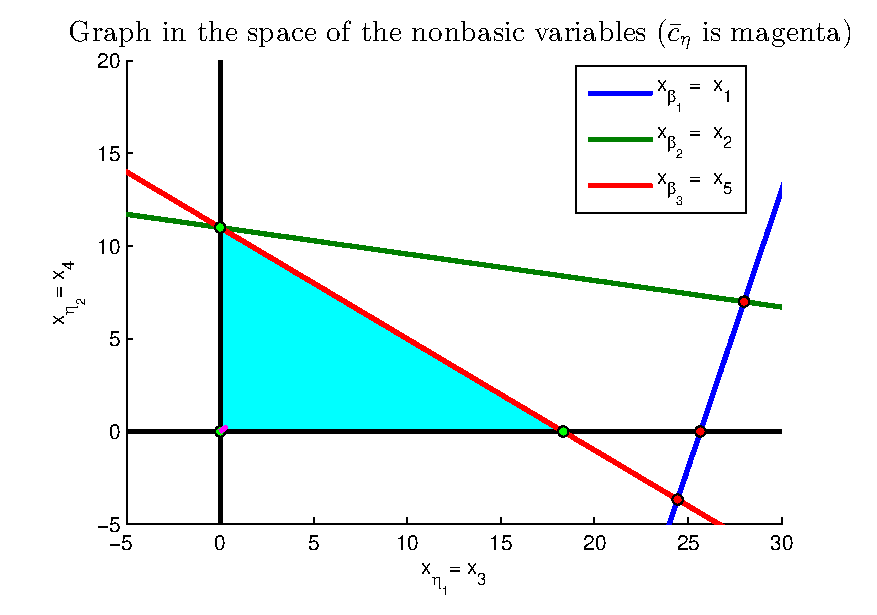
\includegraphics[width=0.5\textwidth]{p6/original.eps}
\caption{Feasible region projected into the space of $(x_3,x_4)$ (original)}\label{fig:p1}
\end{figure}

\begin{figure}[h!!]

\includegraphics[width=0.5\textwidth]{p6/image.eps}
\caption{Feasible region projected into the space of $(x_3,x_4)$ (Gom cuts)}\label{fig:p2}
\end{figure}
